\section{Introduction and System Overview}
\label{sec:Intro}

Configuration errors are one of the most important root-causes of
modern software system failures~\cite{xu15systems,yin11anempirical}.
In practice, misconfiguration problems may result in security
vulnerabilities, application crashes, severe disruptions in software
functionality, and incorrect program executions%
~\cite{xu15systems,zhang14encore,yuan11context}.  Although several
tools have been proposed to automate configuration error diagnosis
after failures occur~\cite{wang04automatic,attariyan10automating,
su07autobash,whitaker04configuration}, these tools rely on manual ways
  to understand and detect the failure symptoms. The main reasons are:
  1) entries in configuration files are untyped assignments, 2) there
  is no explicit structure policy for the entries in configuration
  files, and 3) there is surprisingly little rules specifying the
  entries' constraints.

We propose an approach to the verification of  
configuration files which is based on learning rules about the language 
model for configuration files. 

\begin{figure}[t] \centering
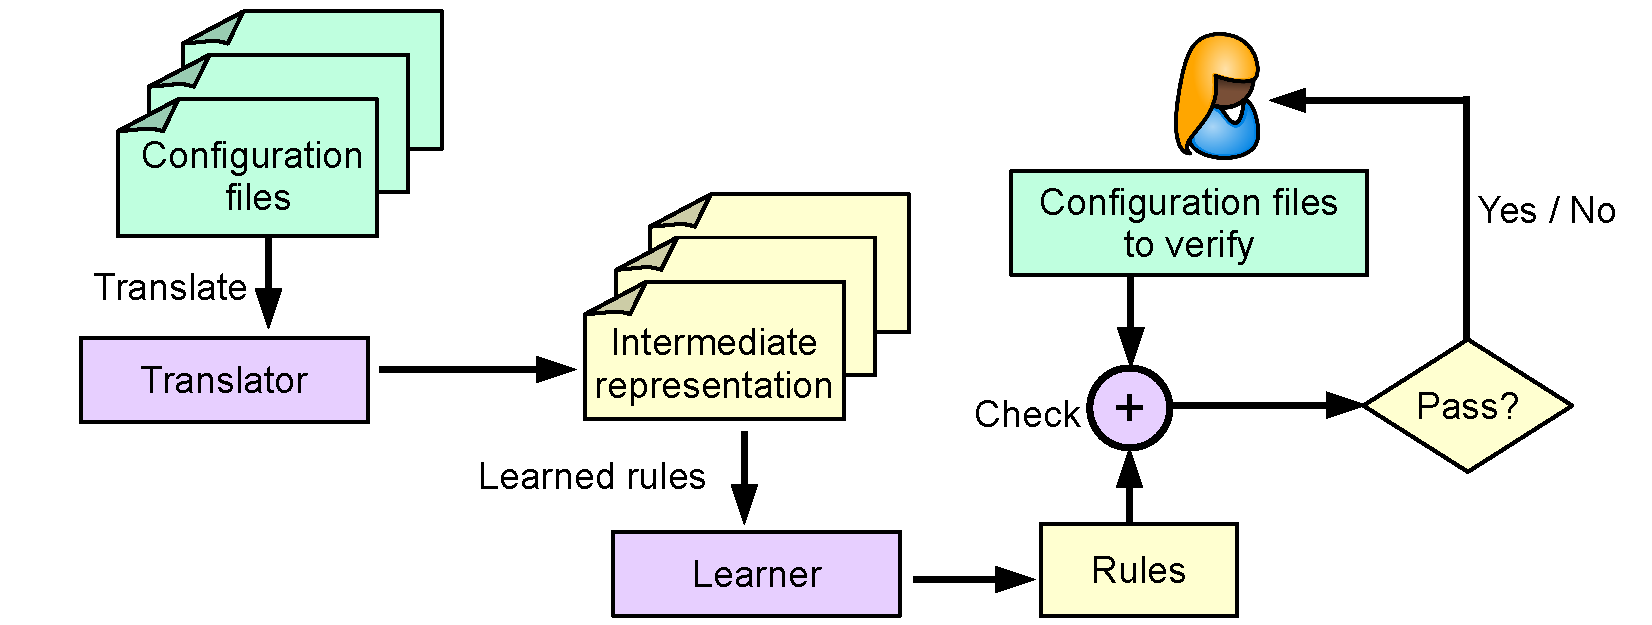
\includegraphics[width=0.8\textwidth]{figs/overview}
\caption{An overview of the \app's workflow.}
\label{fig-overview}
\end{figure}

Fig.~\ref{fig-overview} describes an overview of our system. We start
with an assumption that we are given a number of correct configuration
files belonging to the same category (for instance, MySQL or
Apache). Such files follow the same naming conventions and we use that
fact in a learning algorithm which will result with the rules
describing the language model used in the files. Since the
``language'' of configuration types is untyped and unstructured, we
first parse the files and translate them into a more structured,
typed, intermediary representation. Having more structured files, we
use them as a training set to learn the rules. The learning algorithm
is template-based. We provide an initial set of templates and the
learner learns some concrete instances from the training set. These
rules are used for detecting errors violating the learned constraints
in the files given by the user.

As an 
illustration for a simple rule that we can learn, consider a template is $X_1 \le X_2$, where $X_1$ and $X_2$ are
integer variables. The learned might derive the rule stating that
$\texttt{mysql.max\_persistent} \le \texttt{max\_connections}$. There is a classification and taxonomy of configuration errors in the 
existing work on automated configuration troubleshooting~\cite{yin11anempirical, configdataset}. We provide templates for every class that \app can handle: we consider integer constraints, ordering
constraints, typing constraints, constraints about correlated entries (such as ``if $X$ is present, $Y$ has to appear as well''). Unfortunately, there are a few classes of errors that we cannot handle. They
 rely on the analysis of the whole operating system and our language-based
approach is not expressive enough for them. 

From a  practical perspective there is no additional burden 
to the users: they can simply use \app to check for errors in their configuration files. However, they can also easily extend the framework themselves. The system is designed to be highly modular. If there is a class of rules that \app is not currently learning, the user can develop their own templates and learners for that class. The new learner can be added to \app and this way it can check additionally a new set of errors.

Finally, from a system perspective this is the first approach that checks 
proactively the correctness of configuration files. All previous work
~\cite{xu15systems,zhang14encore,yuan11context, wang04automatic,attariyan10automating,
su07autobash,whitaker04configuration} tries to identify the problem after the
failure occurs. Our approach isolates potential errors before the system failure occurs, e.g. before the installation. We can also see \app as a tool that can run in conjunction with existing tool. Pre-analyzed configuration files are already free from language-based errors, and this way the workloads of post-failure forensics at the runtime
is significantly reduced, thus making these tools truly practical.

Using these ideas, we make the following contributions:

\begin{enumerate}

  \item We designed and implemented a tool, \app, that can learn a language model from a set of examples of correct configuration files, and use the model to verify new files.
  \item We use a probabilistic type that can be used to assign a confidence distribution over a set of types to a value.
  \item In \app, we define a minimal interface for describing a verification attribute in a learning context, making it easy to add new rules to the system.

\end{enumerate}
